% SenHAT architecture diagram — clean, slide-ready
% Compile: pdflatex senhat_architecture.tex
\documentclass[tikz,border=6pt]{standalone}
\usepackage{tikz}
\usetikzlibrary{arrows.meta,positioning,calc,shadows.blur}

\definecolor{DeepBlue}{RGB}{22,58,92}
\definecolor{Accent}{RGB}{0,110,150}
\definecolor{Green}{RGB}{95,155,110}
\definecolor{Orange}{RGB}{210,130,70}
\definecolor{BoxFill}{RGB}{238,244,252}

\tikzset{
  arr/.style={-{Latex[length=3mm,width=2.2mm]}, line width=1.4pt, draw=DeepBlue},
  box/.style={
    draw=DeepBlue, line width=1.1pt, rounded corners=4pt,
    fill=BoxFill, align=center, font=\sffamily\small
  },
  label/.style={font=\sffamily\bfseries\small, text=DeepBlue},
  sublabel/.style={font=\sffamily\footnotesize, text=DeepBlue!80},
}

% Simple isometric feature-map stack (front face + depth offset)
\newcommand{\stack}[6]{%
  % #1=x, #2=y, #3=width, #4=height, #5=layers, #6=face color
  \begin{scope}[shift={(#1,#2)}]
    \pgfmathsetmacro{\dx}{0.22}
    \pgfmathsetmacro{\dy}{0.16}
    \foreach \i in {1,...,#5} {
      \pgfmathsetmacro{\offx}{\i*\dx}
      \pgfmathsetmacro{\offy}{\i*\dy}
      \draw[draw=DeepBlue!70, fill=#6!18, line width=0.6pt]
        ($ (0,0) + (\offx,\offy) $) --
        ($ (#3,0) + (\offx,\offy) $) --
        ($ (#3,#4) + (\offx,\offy) $) --
        ($ (0,#4) + (\offx,\offy) $) -- cycle;
    }
    \draw[draw=DeepBlue, fill=#6!35, line width=1pt]
      (0,0) rectangle (#3,#4);
  \end{scope}
}

\begin{document}
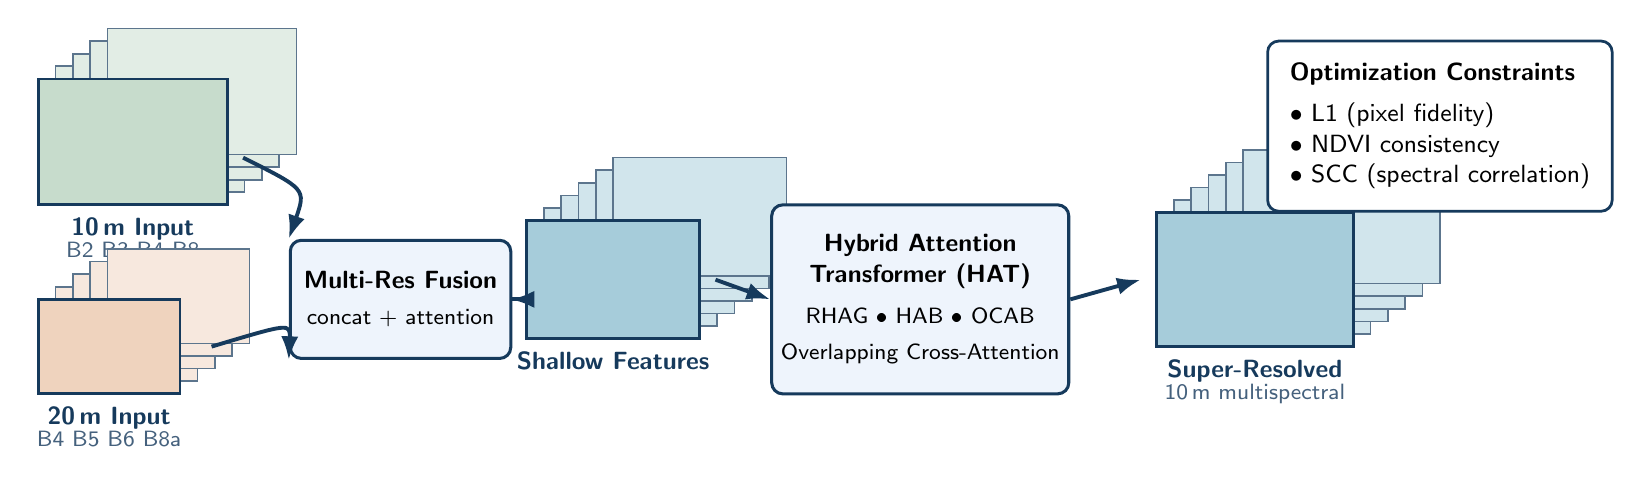
\begin{tikzpicture}[x=1cm,y=1cm]

% ---- Inputs ----
\stack{0}{2.2}{2.4}{1.6}{4}{Green}
\node[label, anchor=north] at (1.2,2.15) {10\,m Input};
\node[sublabel, anchor=north] at (1.2,1.85) {B2 B3 B4 B8};

\stack{0}{-0.2}{1.8}{1.2}{4}{Orange}
\node[label, anchor=north] at (0.9,-0.25) {20\,m Input};
\node[sublabel, anchor=north] at (0.9,-0.55) {B4 B5 B6 B8a};

% ---- Fusion ----
\node[box, minimum width=2.8cm, minimum height=1.5cm] (fuse) at (4.6,1.0)
  {\textbf{Multi-Res Fusion}\\[2pt]\footnotesize concat + attention};

% ---- Shallow features ----
\stack{6.2}{0.5}{2.2}{1.5}{5}{Accent}
\node[label, anchor=north] at (7.3,0.45) {Shallow Features};

% ---- HAT ----
\node[box, minimum width=3.6cm, minimum height=2.4cm] (hat) at (11.2,1.0) {
  \textbf{Hybrid Attention}\\\textbf{Transformer (HAT)}\\[4pt]
  \footnotesize RHAG \textbullet\ HAB \textbullet\ OCAB\\[2pt]
  \footnotesize Overlapping Cross-Attention
};

% ---- Output ----
\stack{14.2}{0.4}{2.5}{1.7}{5}{Accent}
\node[label, anchor=north] at (15.45,0.35) {Super-Resolved};
\node[sublabel, anchor=north] at (15.45,0.05) {10\,m multispectral};

% ---- Arrows ----
\draw[arr] (2.6,2.8) .. controls (3.4,2.4) .. (fuse.north west);
\draw[arr] (2.2,0.4) .. controls (3.2,0.7) .. (fuse.south west);
\draw[arr] (fuse.east) -- (6.0,1.0);
\draw[arr] (8.6,1.25) -- (hat.west);
\draw[arr] (hat.east) -- (14.0,1.25);

% ---- Loss constraints (right panel) ----
\node[
  draw=DeepBlue, line width=1pt, rounded corners=4pt,
  fill=white, align=left, font=\sffamily\small,
  inner sep=8pt
] at (17.8,3.2) {
  \textbf{Optimization Constraints}\\[4pt]
  $\bullet$ L1 (pixel fidelity)\\
  $\bullet$ NDVI consistency\\
  $\bullet$ SCC (spectral correlation)
};

\end{tikzpicture}
\end{document}
